% Content for Quantization Methods subsection
% This file is included in the main conference paper via % Content for Quantization Methods subsection
% This file is included in the main conference paper via % Content for Quantization Methods subsection
% This file is included in the main conference paper via % Content for Quantization Methods subsection
% This file is included in the main conference paper via \input{QuantizationMethods}
\subsubsection{Quantization Theory}
Quantization is the lossy process of reducing the bits needed to store data by dividing  from a larger range of values to a smaller range of values. By decreasing the range used to represent the data, entropy is lowered, as multiple values pre-quantization may be mapped to one value during quantization. With this mapping being many-to-one, this operation cannot be reversed, showing that quantization is necessarily lossy. With the goal of transforms being to decrease entropy while ensuring perfect reconstruction of an image, quantization is used to further improve compression ratio beyond entropy-bound compression used in lossless algorithms, sacrificing image fidelity in the process. Fig. \ref{fig:quantization} depicts the effect of increasing levels of quantization and the associated loss of image quality, along with compression ratio of the compressed file as defined in \ref{sec:intro}.

\begin{figure}
    \centering
    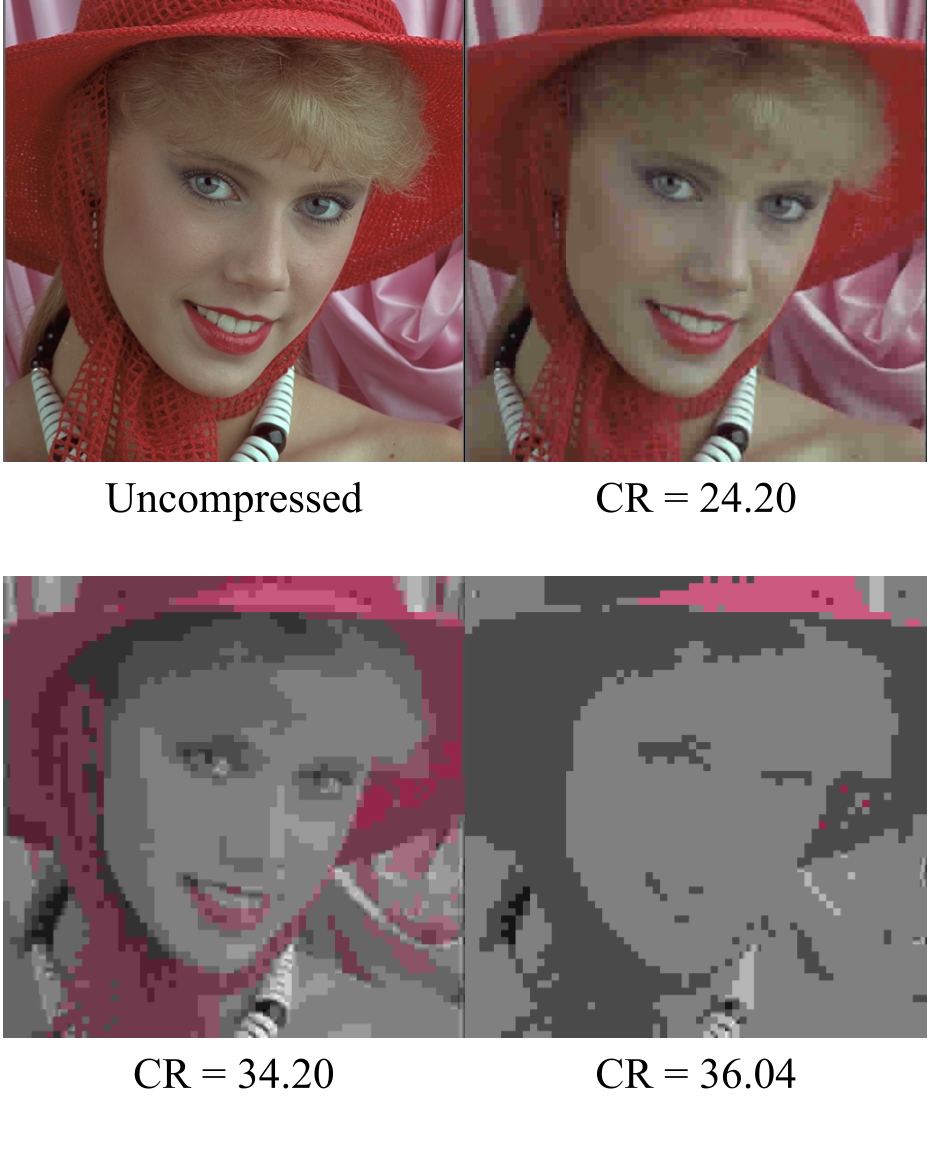
\includegraphics[width=0.8\linewidth]{methods/figures/quantizationfigure.png}
    \caption{Different levels of quantization on sample image with resulting compression ratio.}
    \label{fig:quantization}
\end{figure}

A central component to quantization is step size $\Delta$, which points to the ranges of pre-quantized values that would be quantized to one resulting value. With R representing the range of values and M the number of steps, step size is given by:
\begin{equation}
\Delta = \frac{R}{M}\label{eq}
\end{equation}
To illustrate the role of step size, consider an 8-bit signal whose values lie in the range 0–255. A step size of $\Delta = 2$ would quantize that range into $128$ steps:
\begin{equation}
2 = \frac{256}{M}\label{step_size}
\end{equation}
\begin{equation}
M = 128 = 2^{7}\label{7bits}
\end{equation}
Thus, the output symbols of this example quantizer can be represented using $7$ bits per value, before the following entropy encoding.

In our study, a relatively simple base quantization method was devised based on the JPEG Compression Standard. Quantization was applied on each chunk via division by a defined quantization matrix associated with each transform. DCT and DFT utilized a quantization matrix specified by the JPEG Compression Standard, whereas other transforms had quantization matrices calculated based on transformed data ranges.

Because the JPEG-specified quantization matrix is labeled as resulting in a 50\% reduction in quality, the quantization methods for the Haar and S+P transforms aimed to reduce the theoretical bit-representation of the image from 8 bits to 7 bits. For the Haar transform, this was done by calculating the data ranges for each quadrant of each transformed chunk and choosing the appropriate step sizes based on $M = 128$ to achieve a basic quantization matrix. A unique quantization method was created for the S+P transform. 
\subsubsection{Quantization for the S+P Transform}

For lossy compression, we introduce bandwise scalar quantization on top of the
S+P coefficients. Because S+P already segregates information into subbands of
differing perceptual importance (LL vs.\ HL/LH/HH), it is natural to assign
different step sizes to each band rather than using a uniform matrix.

\paragraph{Bandwise and level-dependent parameterization.}
Our implementation exposes a small set of quantization parameters in a
\texttt{QuantParams} structure:
\begin{itemize}
    \item $q_{\mathrm{LL}}, q_{\mathrm{HL}}, q_{\mathrm{LH}}, q_{\mathrm{HH}}$: base step sizes for the four subbands,
    \item \texttt{deadzone}: a dimensionless multiplier for the central dead-zone,
    \item \texttt{scale}: a global scale factor applied uniformly across bands,
    \item \texttt{level\_gamma}: a geometric multiplier applied per pyramid level.
\end{itemize}

From these we compute per-level step sizes
\begin{align}
    q_{\mathrm{band}}^{(L)} &= \left\lfloor
        \texttt{scale} \cdot \mathrm{level\_factor}(L) \cdot q_{\mathrm{band}}
    \right\rfloor, \\
    \mathrm{level\_factor}(L) &=
      \begin{cases}
        \texttt{level\_gamma}^{L}, & \text{if } \texttt{level\_gamma} > 0, \\
        1, & \text{otherwise}.
      \end{cases}
\end{align}
for each band and level $L$. In practice, the LL band at coarse levels is often
left unquantized or lightly quantized, while higher-frequency bands (HL/LH/HH)
receive progressively larger steps, reflecting their lower perceptual weight.
Because all S+P coefficients are integers, these step sizes are also rounded to
integers, which can further couple quantizer behavior to the underlying
coefficient distribution. As in the Haar case, the choice of \texttt{deadzone}
is made empirically and tuned based on observed rate--distortion behavior.

\paragraph{Dead-zone scalar quantization.}
Within each subband, we apply a standard dead-zone scalar quantizer. Given a
coefficient $x$ and step size $\Delta$, we compute
\begin{equation}
    q =
    \begin{cases}
      0, & |x| < \texttt{deadzone}\cdot\Delta, \\
      \mathrm{sign}(x)\,\left\lfloor \dfrac{|x|}{\Delta} \right\rfloor,
      & \text{otherwise,}
    \end{cases}
\end{equation}
and reconstruct via $\hat{x} = q\Delta$ during decoding. The enlarged dead-zone
encourages small-magnitude coefficients—especially in the highpass bands—to be
quantized to zero, producing longer zero-runs that the entropy coder can
compress efficiently.

Because the S+P transform tends to reduce the variance and entropy of its
highpass residuals, relatively simple scalar quantizers can still achieve a wide
range of operating points. Moreover, the explicit bandwise and level-dependent
parameters allow us to adjust $(q_{\mathrm{LL}}, q_{\mathrm{HL}},
q_{\mathrm{LH}}, q_{\mathrm{HH}})$ and \texttt{level\_gamma} to probe different
rate--distortion regimes without modifying the transform itself.

\subsubsection{Quantization Theory}
Quantization is the lossy process of reducing the bits needed to store data by dividing  from a larger range of values to a smaller range of values. By decreasing the range used to represent the data, entropy is lowered, as multiple values pre-quantization may be mapped to one value during quantization. With this mapping being many-to-one, this operation cannot be reversed, showing that quantization is necessarily lossy. With the goal of transforms being to decrease entropy while ensuring perfect reconstruction of an image, quantization is used to further improve compression ratio beyond entropy-bound compression used in lossless algorithms, sacrificing image fidelity in the process. Fig. \ref{fig:quantization} depicts the effect of increasing levels of quantization and the associated loss of image quality, along with compression ratio of the compressed file as defined in \ref{sec:intro}.

\begin{figure}
    \centering
    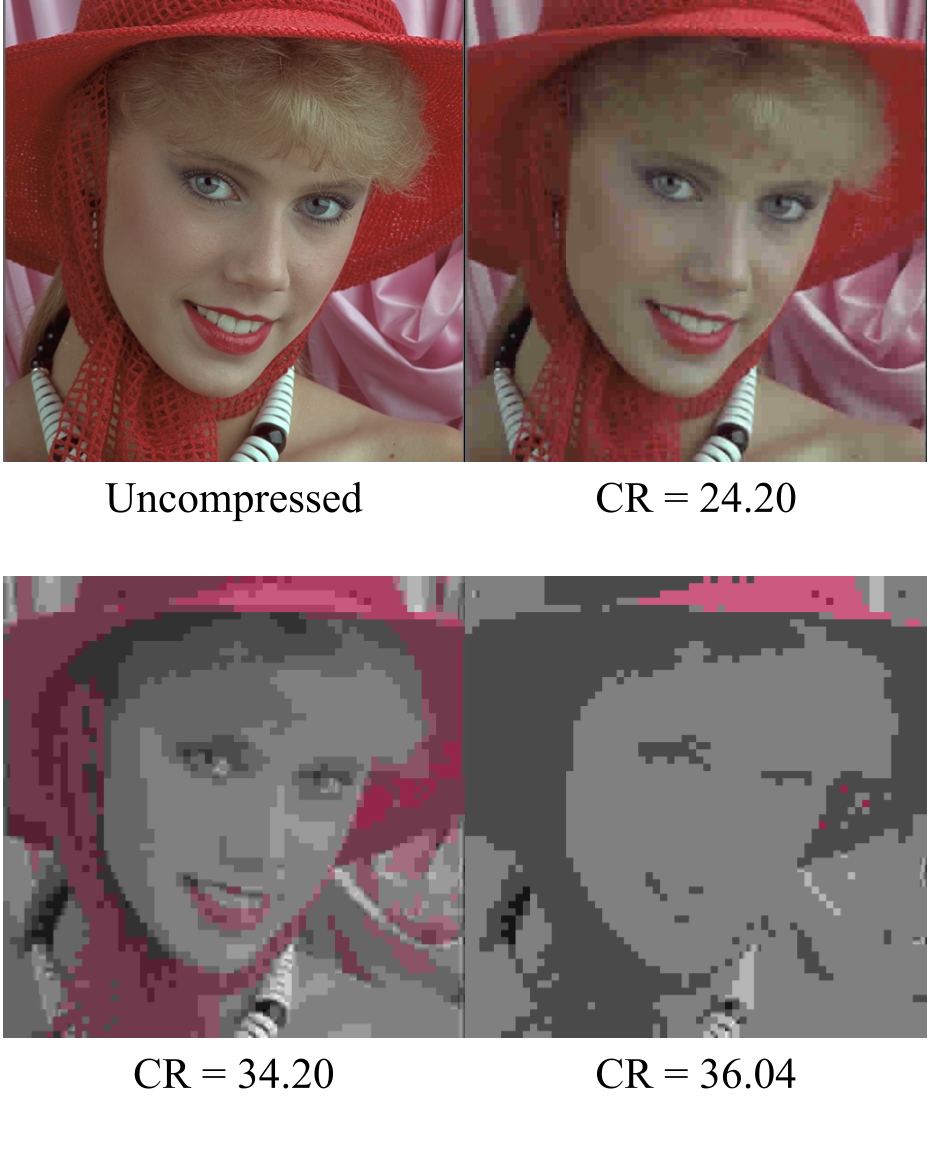
\includegraphics[width=0.8\linewidth]{methods/figures/quantizationfigure.png}
    \caption{Different levels of quantization on sample image with resulting compression ratio.}
    \label{fig:quantization}
\end{figure}

A central component to quantization is step size $\Delta$, which points to the ranges of pre-quantized values that would be quantized to one resulting value. With R representing the range of values and M the number of steps, step size is given by:
\begin{equation}
\Delta = \frac{R}{M}\label{eq}
\end{equation}
To illustrate the role of step size, consider an 8-bit signal whose values lie in the range 0–255. A step size of $\Delta = 2$ would quantize that range into $128$ steps:
\begin{equation}
2 = \frac{256}{M}\label{step_size}
\end{equation}
\begin{equation}
M = 128 = 2^{7}\label{7bits}
\end{equation}
Thus, the output symbols of this example quantizer can be represented using $7$ bits per value, before the following entropy encoding.

In our study, a relatively simple base quantization method was devised based on the JPEG Compression Standard. Quantization was applied on each chunk via division by a defined quantization matrix associated with each transform. DCT and DFT utilized a quantization matrix specified by the JPEG Compression Standard, whereas other transforms had quantization matrices calculated based on transformed data ranges.

Because the JPEG-specified quantization matrix is labeled as resulting in a 50\% reduction in quality, the quantization methods for the Haar and S+P transforms aimed to reduce the theoretical bit-representation of the image from 8 bits to 7 bits. For the Haar transform, this was done by calculating the data ranges for each quadrant of each transformed chunk and choosing the appropriate step sizes based on $M = 128$ to achieve a basic quantization matrix. A unique quantization method was created for the S+P transform. 
\subsubsection{Quantization for the S+P Transform}

For lossy compression, we introduce bandwise scalar quantization on top of the
S+P coefficients. Because S+P already segregates information into subbands of
differing perceptual importance (LL vs.\ HL/LH/HH), it is natural to assign
different step sizes to each band rather than using a uniform matrix.

\paragraph{Bandwise and level-dependent parameterization.}
Our implementation exposes a small set of quantization parameters in a
\texttt{QuantParams} structure:
\begin{itemize}
    \item $q_{\mathrm{LL}}, q_{\mathrm{HL}}, q_{\mathrm{LH}}, q_{\mathrm{HH}}$: base step sizes for the four subbands,
    \item \texttt{deadzone}: a dimensionless multiplier for the central dead-zone,
    \item \texttt{scale}: a global scale factor applied uniformly across bands,
    \item \texttt{level\_gamma}: a geometric multiplier applied per pyramid level.
\end{itemize}

From these we compute per-level step sizes
\begin{align}
    q_{\mathrm{band}}^{(L)} &= \left\lfloor
        \texttt{scale} \cdot \mathrm{level\_factor}(L) \cdot q_{\mathrm{band}}
    \right\rfloor, \\
    \mathrm{level\_factor}(L) &=
      \begin{cases}
        \texttt{level\_gamma}^{L}, & \text{if } \texttt{level\_gamma} > 0, \\
        1, & \text{otherwise}.
      \end{cases}
\end{align}
for each band and level $L$. In practice, the LL band at coarse levels is often
left unquantized or lightly quantized, while higher-frequency bands (HL/LH/HH)
receive progressively larger steps, reflecting their lower perceptual weight.
Because all S+P coefficients are integers, these step sizes are also rounded to
integers, which can further couple quantizer behavior to the underlying
coefficient distribution. As in the Haar case, the choice of \texttt{deadzone}
is made empirically and tuned based on observed rate--distortion behavior.

\paragraph{Dead-zone scalar quantization.}
Within each subband, we apply a standard dead-zone scalar quantizer. Given a
coefficient $x$ and step size $\Delta$, we compute
\begin{equation}
    q =
    \begin{cases}
      0, & |x| < \texttt{deadzone}\cdot\Delta, \\
      \mathrm{sign}(x)\,\left\lfloor \dfrac{|x|}{\Delta} \right\rfloor,
      & \text{otherwise,}
    \end{cases}
\end{equation}
and reconstruct via $\hat{x} = q\Delta$ during decoding. The enlarged dead-zone
encourages small-magnitude coefficients—especially in the highpass bands—to be
quantized to zero, producing longer zero-runs that the entropy coder can
compress efficiently.

Because the S+P transform tends to reduce the variance and entropy of its
highpass residuals, relatively simple scalar quantizers can still achieve a wide
range of operating points. Moreover, the explicit bandwise and level-dependent
parameters allow us to adjust $(q_{\mathrm{LL}}, q_{\mathrm{HL}},
q_{\mathrm{LH}}, q_{\mathrm{HH}})$ and \texttt{level\_gamma} to probe different
rate--distortion regimes without modifying the transform itself.

\subsubsection{Quantization Theory}
Quantization is the lossy process of reducing the bits needed to store data by dividing  from a larger range of values to a smaller range of values. By decreasing the range used to represent the data, entropy is lowered, as multiple values pre-quantization may be mapped to one value during quantization. With this mapping being many-to-one, this operation cannot be reversed, showing that quantization is necessarily lossy. With the goal of transforms being to decrease entropy while ensuring perfect reconstruction of an image, quantization is used to further improve compression ratio beyond entropy-bound compression used in lossless algorithms, sacrificing image fidelity in the process. Fig. \ref{fig:quantization} depicts the effect of increasing levels of quantization and the associated loss of image quality, along with compression ratio of the compressed file as defined in \ref{sec:intro}.

\begin{figure}
    \centering
    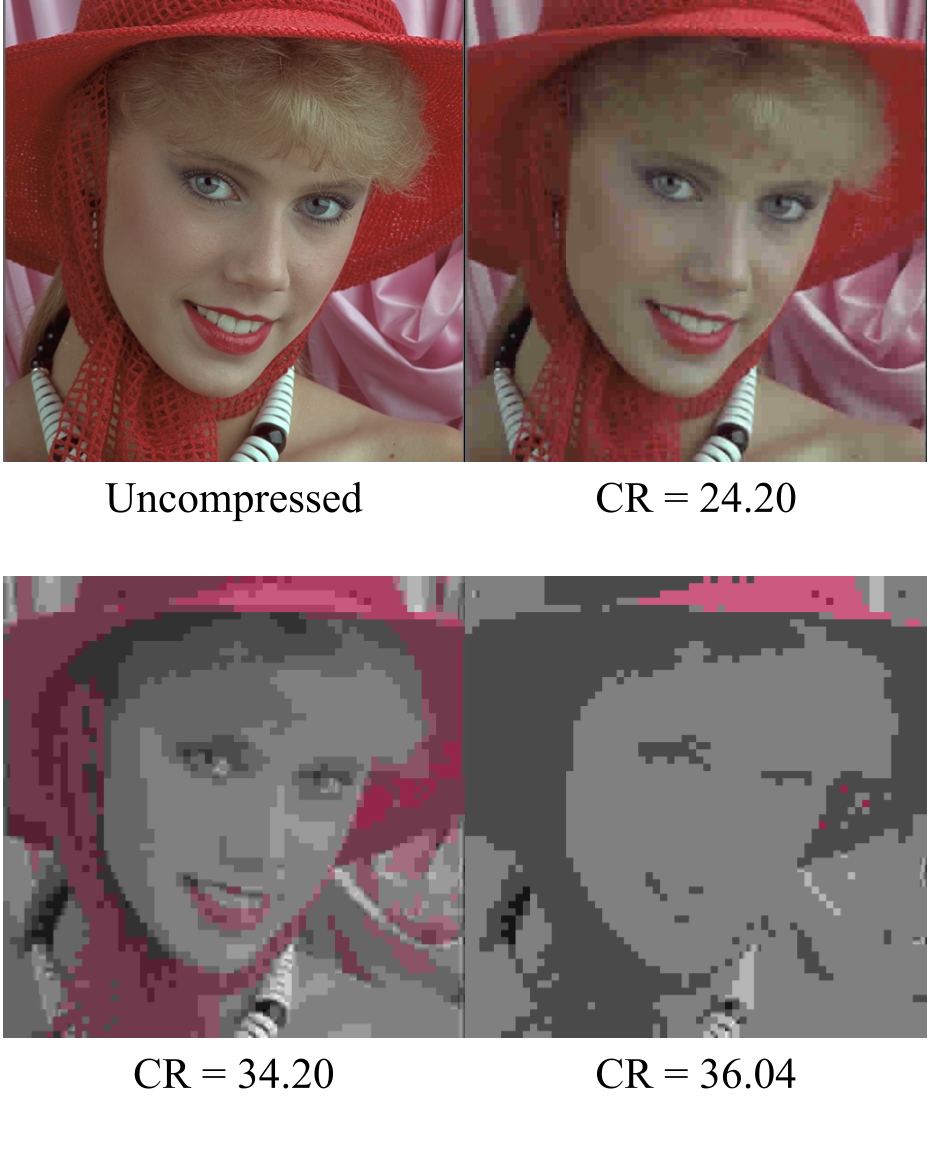
\includegraphics[width=0.8\linewidth]{methods/figures/quantizationfigure.png}
    \caption{Different levels of quantization on sample image with resulting compression ratio.}
    \label{fig:quantization}
\end{figure}

A central component to quantization is step size $\Delta$, which points to the ranges of pre-quantized values that would be quantized to one resulting value. With R representing the range of values and M the number of steps, step size is given by:
\begin{equation}
\Delta = \frac{R}{M}\label{eq}
\end{equation}
To illustrate the role of step size, consider an 8-bit signal whose values lie in the range 0–255. A step size of $\Delta = 2$ would quantize that range into $128$ steps:
\begin{equation}
2 = \frac{256}{M}\label{step_size}
\end{equation}
\begin{equation}
M = 128 = 2^{7}\label{7bits}
\end{equation}
Thus, the output symbols of this example quantizer can be represented using $7$ bits per value, before the following entropy encoding.

In our study, a relatively simple base quantization method was devised based on the JPEG Compression Standard. Quantization was applied on each chunk via division by a defined quantization matrix associated with each transform. DCT and DFT utilized a quantization matrix specified by the JPEG Compression Standard, whereas other transforms had quantization matrices calculated based on transformed data ranges.

Because the JPEG-specified quantization matrix is labeled as resulting in a 50\% reduction in quality, the quantization methods for the Haar and S+P transforms aimed to reduce the theoretical bit-representation of the image from 8 bits to 7 bits. For the Haar transform, this was done by calculating the data ranges for each quadrant of each transformed chunk and choosing the appropriate step sizes based on $M = 128$ to achieve a basic quantization matrix. A unique quantization method was created for the S+P transform. 
\subsubsection{Quantization for the S+P Transform}

For lossy compression, we introduce bandwise scalar quantization on top of the
S+P coefficients. Because S+P already segregates information into subbands of
differing perceptual importance (LL vs.\ HL/LH/HH), it is natural to assign
different step sizes to each band rather than using a uniform matrix.

\paragraph{Bandwise and level-dependent parameterization.}
Our implementation exposes a small set of quantization parameters in a
\texttt{QuantParams} structure:
\begin{itemize}
    \item $q_{\mathrm{LL}}, q_{\mathrm{HL}}, q_{\mathrm{LH}}, q_{\mathrm{HH}}$: base step sizes for the four subbands,
    \item \texttt{deadzone}: a dimensionless multiplier for the central dead-zone,
    \item \texttt{scale}: a global scale factor applied uniformly across bands,
    \item \texttt{level\_gamma}: a geometric multiplier applied per pyramid level.
\end{itemize}

From these we compute per-level step sizes
\begin{align}
    q_{\mathrm{band}}^{(L)} &= \left\lfloor
        \texttt{scale} \cdot \mathrm{level\_factor}(L) \cdot q_{\mathrm{band}}
    \right\rfloor, \\
    \mathrm{level\_factor}(L) &=
      \begin{cases}
        \texttt{level\_gamma}^{L}, & \text{if } \texttt{level\_gamma} > 0, \\
        1, & \text{otherwise}.
      \end{cases}
\end{align}
for each band and level $L$. In practice, the LL band at coarse levels is often
left unquantized or lightly quantized, while higher-frequency bands (HL/LH/HH)
receive progressively larger steps, reflecting their lower perceptual weight.
Because all S+P coefficients are integers, these step sizes are also rounded to
integers, which can further couple quantizer behavior to the underlying
coefficient distribution. As in the Haar case, the choice of \texttt{deadzone}
is made empirically and tuned based on observed rate--distortion behavior.

\paragraph{Dead-zone scalar quantization.}
Within each subband, we apply a standard dead-zone scalar quantizer. Given a
coefficient $x$ and step size $\Delta$, we compute
\begin{equation}
    q =
    \begin{cases}
      0, & |x| < \texttt{deadzone}\cdot\Delta, \\
      \mathrm{sign}(x)\,\left\lfloor \dfrac{|x|}{\Delta} \right\rfloor,
      & \text{otherwise,}
    \end{cases}
\end{equation}
and reconstruct via $\hat{x} = q\Delta$ during decoding. The enlarged dead-zone
encourages small-magnitude coefficients—especially in the highpass bands—to be
quantized to zero, producing longer zero-runs that the entropy coder can
compress efficiently.

Because the S+P transform tends to reduce the variance and entropy of its
highpass residuals, relatively simple scalar quantizers can still achieve a wide
range of operating points. Moreover, the explicit bandwise and level-dependent
parameters allow us to adjust $(q_{\mathrm{LL}}, q_{\mathrm{HL}},
q_{\mathrm{LH}}, q_{\mathrm{HH}})$ and \texttt{level\_gamma} to probe different
rate--distortion regimes without modifying the transform itself.

\subsubsection{Quantization Theory}
Quantization is the lossy process of reducing the bits needed to store data by dividing  from a larger range of values to a smaller range of values. By decreasing the range used to represent the data, entropy is lowered, as multiple values pre-quantization may be mapped to one value during quantization. With this mapping being many-to-one, this operation cannot be reversed, showing that quantization is necessarily lossy. With the goal of transforms being to decrease entropy while ensuring perfect reconstruction of an image, quantization is used to further improve compression ratio beyond entropy-bound compression used in lossless algorithms, sacrificing image fidelity in the process. Fig. \ref{fig:quantization} depicts the effect of increasing levels of quantization and the associated loss of image quality, along with compression ratio of the compressed file as defined in \ref{sec:intro}.

\begin{figure}
    \centering
    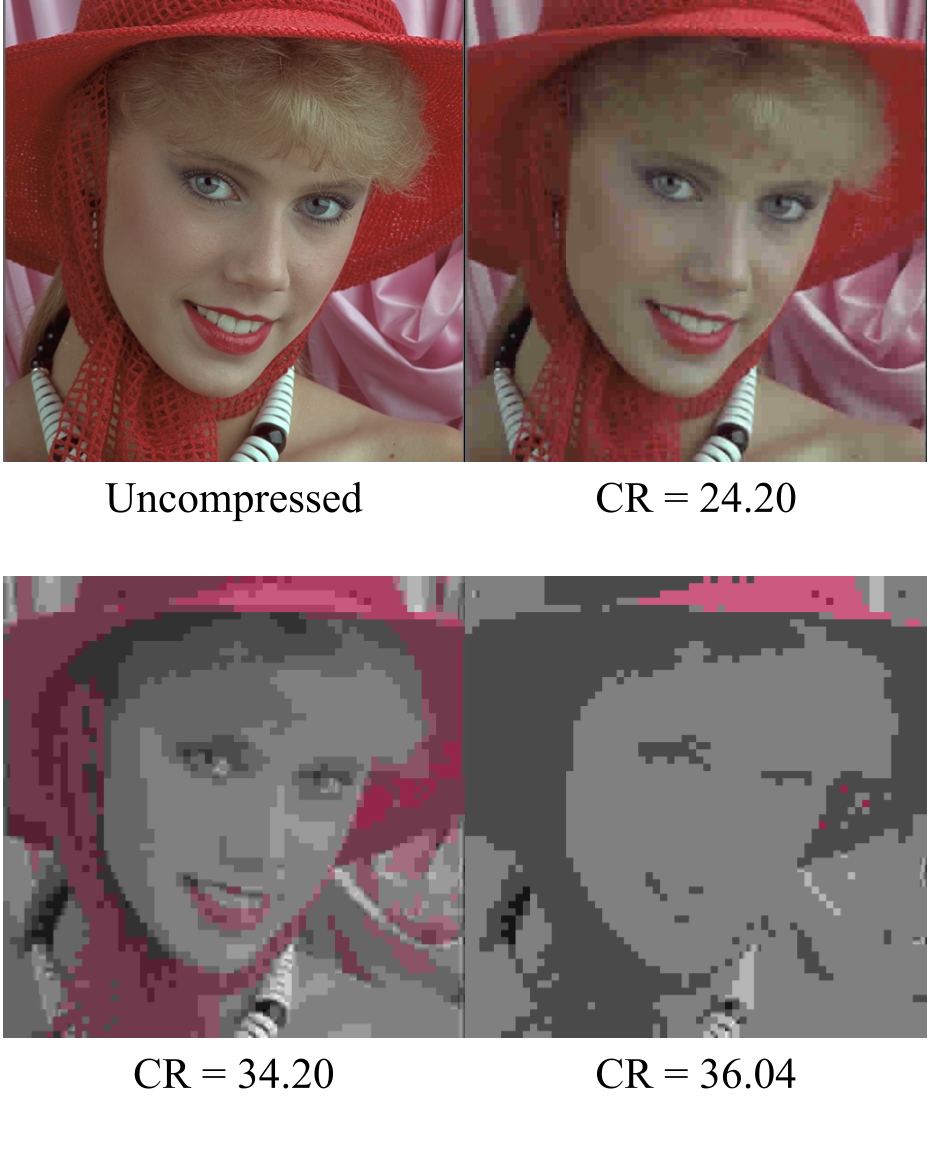
\includegraphics[width=0.8\linewidth]{methods/figures/quantizationfigure.png}
    \caption{Different levels of quantization on sample image with resulting compression ratio.}
    \label{fig:quantization}
\end{figure}

A central component to quantization is step size $\Delta$, which points to the ranges of pre-quantized values that would be quantized to one resulting value. With R representing the range of values and M the number of steps, step size is given by:
\begin{equation}
\Delta = \frac{R}{M}\label{eq}
\end{equation}
To illustrate the role of step size, consider an 8-bit signal whose values lie in the range 0–255. A step size of $\Delta = 2$ would quantize that range into $128$ steps:
\begin{equation}
2 = \frac{256}{M}\label{step_size}
\end{equation}
\begin{equation}
M = 128 = 2^{7}\label{7bits}
\end{equation}
Thus, the output symbols of this example quantizer can be represented using $7$ bits per value, before the following entropy encoding.

In our study, a relatively simple base quantization method was devised based on the JPEG Compression Standard. Quantization was applied on each chunk via division by a defined quantization matrix associated with each transform. DCT and DFT utilized a quantization matrix specified by the JPEG Compression Standard, whereas other transforms had quantization matrices calculated based on transformed data ranges.

Because the JPEG-specified quantization matrix is labeled as resulting in a 50\% reduction in quality, the quantization methods for the Haar and S+P transforms aimed to reduce the theoretical bit-representation of the image from 8 bits to 7 bits. For the Haar transform, this was done by calculating the data ranges for each quadrant of each transformed chunk and choosing the appropriate step sizes based on $M = 128$ to achieve a basic quantization matrix. A unique quantization method was created for the S+P transform. 
\subsubsection{Quantization for the S+P Transform}

For lossy compression, we introduce bandwise scalar quantization on top of the
S+P coefficients. Because S+P already segregates information into subbands of
differing perceptual importance (LL vs.\ HL/LH/HH), it is natural to assign
different step sizes to each band rather than using a uniform matrix.

\paragraph{Bandwise and level-dependent parameterization.}
Our implementation exposes a small set of quantization parameters in a
\texttt{QuantParams} structure:
\begin{itemize}
    \item $q_{\mathrm{LL}}, q_{\mathrm{HL}}, q_{\mathrm{LH}}, q_{\mathrm{HH}}$: base step sizes for the four subbands,
    \item \texttt{deadzone}: a dimensionless multiplier for the central dead-zone,
    \item \texttt{scale}: a global scale factor applied uniformly across bands,
    \item \texttt{level\_gamma}: a geometric multiplier applied per pyramid level.
\end{itemize}

From these we compute per-level step sizes
\begin{align}
    q_{\mathrm{band}}^{(L)} &= \left\lfloor
        \texttt{scale} \cdot \mathrm{level\_factor}(L) \cdot q_{\mathrm{band}}
    \right\rfloor, \\
    \mathrm{level\_factor}(L) &=
      \begin{cases}
        \texttt{level\_gamma}^{L}, & \text{if } \texttt{level\_gamma} > 0, \\
        1, & \text{otherwise}.
      \end{cases}
\end{align}
for each band and level $L$. In practice, the LL band at coarse levels is often
left unquantized or lightly quantized, while higher-frequency bands (HL/LH/HH)
receive progressively larger steps, reflecting their lower perceptual weight.
Because all S+P coefficients are integers, these step sizes are also rounded to
integers, which can further couple quantizer behavior to the underlying
coefficient distribution. As in the Haar case, the choice of \texttt{deadzone}
is made empirically and tuned based on observed rate--distortion behavior.

\paragraph{Dead-zone scalar quantization.}
Within each subband, we apply a standard dead-zone scalar quantizer. Given a
coefficient $x$ and step size $\Delta$, we compute
\begin{equation}
    q =
    \begin{cases}
      0, & |x| < \texttt{deadzone}\cdot\Delta, \\
      \mathrm{sign}(x)\,\left\lfloor \dfrac{|x|}{\Delta} \right\rfloor,
      & \text{otherwise,}
    \end{cases}
\end{equation}
and reconstruct via $\hat{x} = q\Delta$ during decoding. The enlarged dead-zone
encourages small-magnitude coefficients—especially in the highpass bands—to be
quantized to zero, producing longer zero-runs that the entropy coder can
compress efficiently.

Because the S+P transform tends to reduce the variance and entropy of its
highpass residuals, relatively simple scalar quantizers can still achieve a wide
range of operating points. Moreover, the explicit bandwise and level-dependent
parameters allow us to adjust $(q_{\mathrm{LL}}, q_{\mathrm{HL}},
q_{\mathrm{LH}}, q_{\mathrm{HH}})$ and \texttt{level\_gamma} to probe different
rate--distortion regimes without modifying the transform itself.
